



% Chapter 

\chapter{Towards more Complex Models} % Chapter title

\label{ch:complexmodels} % For referencing the chapter elsewhere, use \autoref{ch:name} 


%----------------------------------------------------------------------------------------

This single section chapter is differentiated from the previous one as it makes a step further towards more complex models. A toy-model introducing governance processes is described. Such exploration logically enters our theoretical framework to try to validate or invalidate the network necessity assumption : if non-linear necessary processes are highlighted and validated against stylized facts, it argues towards the validation of this assumption. 

Other targeted projects such as the exploration of an hybrid macro-economic/accessibility-based model to explore transportation companies line implementation strategies are still at the state of ideas and are not described here.



%----------------------------------------------------------------------------------------


\section[The Lutecia Model]{Taking Governance into account in Network Production Processes : The Lutecia Model}


%%%%%%%%%%%%%%%%%%
\subsection{Thematic Context}


We briefly describe a simple game-theory based framework, conjointly done with \noun{Le Nechet} which aims to be integrated as behavioral rules for governing agents in a hybrid model introduced in~\cite{le2010approche} and formalized then explored in~\cite{lenechet2012}. This model couples land-use dynamics with transportation infrastructure evolution and aims to endogeneize transportation infrastructure development at different levels. The framework proposed extends it by allowing cooperation and fusion between governing entities.



As detailed in~\cite{lenechet2012}, a conceptual city system with local administrative boundaries and corresponding governing agents (mayors), and a global governor (state) is the foundation of the model. A land-use evolution (residences and employments localisations) and transportation (gravity flows) are the first step of an iteration. The transportation infrastructure (road network) is then evolved by constructing a new road. First level of decision (global or local) is chosen randomly according to a fixed probability, and in the case of a local decision, the richest mayor will build the new road. The road is then build optimizing the marginal accessibility for the area corresponding to the builder in charge (all world if global, commun if local).

One thematic aspect lacking in the model and that would be interesting to study is the emergence of larger administrative zones, i.e. the emergence of new levels of governance in polycentric metropolitan areas. The reality is of course not as simple, as bottom-up initiatives such as collaboration between neighbor cities are interlaced with top-down decisions such as e.g. the ``M{\'e}tropole du Grand Paris'' which is a new administrative structure for Paris Area decided at the state level~\cite{gilli2009paris}. It would be however interesting to test conditions for emergence of governance patterns from the bottom-up in a conceptual way by extending the model and adding interactions and fusion between administrative entities.

The extension shall consist in relaxing the assumption of a single road segment built at each time step and attribute one segment to the $N$ richest mayors. That leads to situation where neighbor towns may want to construct both a new road. As they are likely to communicate with each other, we assume that negotiations take place and that they consider eventually to build in common, in which case they merge after (rough simplifying but stylized assumption). Such negotiations may be interpreted as a game in the sense of Game Theory, which as already been widely applied for modeling in social and political sciences for questions dealing with cognitive interacting agents with individual interests~\cite{ordeshook1986game}. Such a framework as already been used in transportation investment studies, as e.g. in~\cite{Roumboutsos2008209} where choices of operators (public and privates) to integrate their system in a global consistent commuter system is explored through the notion of Nash equilibrium.

% \cite{2016arXiv161208111S} : rationale for staying at two players : games with many become chaotic




\subsection{Formalization}


The model architecture couples in a complex way a module for land-use evolution with a module for transportation network growth. Submodules, detailed in the following, include in particular a governance module that rules processes of network evolution.


\subsubsection{Land-use evolution}

The following steps are detailed in~\cite{lenechet2012} but we recall the big picture :

\begin{itemize}
\item Initial distribution of Actives and Employments is done around governance centers at positions $\vec{x}_i$ by
\[
A(\vec{x}) = A_{max} \cdot \exp{\left(\frac{\norm{\vec{x}-\vec{x}_i}}{r_A}\right)} ; 
E(\vec{x}) = E_{max} \cdot \exp{\left(\frac{\norm{\vec{x}-\vec{x}_i}}{r_E}\right)}
\]

\item For facility patches, employments are added by $E(\vec{x}) = E(\vec{x})+\frac{k_{ext}\cdot E_{max}}{n_{ext}}$.

\item Transportation module : computation of flows $\phi_{ij}$ are done by solving on $p_i,q_j$ by a fixed point method (Furness algorithm), the system of gravity flows
\[
\begin{cases}
\phi_{ij} = p_i q_j A_i E_j \exp{\left(-\lambda_{tr} d_{ij}\right)}\\
\sum_k \phi_{kj} = E_j ; \sum_k \phi_{ik} = A_i\\
p_i = \frac{1}{\sum_k{q_k E_k \exp{(-\lambda_{tr}d_{ik})}}} ; q_j = \frac{1}{\sum_k{p_k A_k \exp{(-\lambda_{tr}d_{kj})}}} 
\end{cases}
\]

\item Trajectories then attributed by effective shortest path, and corresponding congestion $c$ obtained (no Wardrop equilibrium). 

\item Speed of network is given by a BPR function $v(c) = v_0 \left(1 - \frac{c}{\kappa}\right)^{\gamma_c}$. Congestion is not used in current studies (infinite capacity $\kappa$).

\item Land-Use module : we assume that residential/employments relocations are at equilibrium at the time scale of a tick, that corresponds to transportation infrastructure evolution time scale which is much larger~\cite{bretagnolle:tel-00459720}.

\item We take a Cobb-douglas function for utilities of actives/employments at a given cell
\[
U_i (A) = X_i(A)^{\gamma_A}\cdot {F_i(A)}^{1-\gamma_A} ; F_i(A) = \frac{1}{A_i E_i}
\]
\[
U_j (E) = X_j(E)^{\gamma_E}\cdot {F_j(E)}^{1-\gamma_E} ; F_j(E) = 1
\]

where $X_i(A) = A_i\cdot \sum_j{E_j \exp{\left(-\lambda\cdot d_{ij}\right)}}$ and $X_j(E) = E_j\cdot \sum_i{A_i \exp{\left(-\lambda\cdot d_{ij}\right)}}$.

\item Relocations are then done deterministically following a discrete choice model :
\[
A_i(t+1) = \sum_i{A_i(t)}\cdot\frac{\exp{(\beta U_i(A))}}{\sum_i{\exp{(\beta U_i(A))}}}
\]
\[
E_j(t+1) = \sum_j{E_j(t)}\cdot\frac{\exp{(\beta U_j(E))}}{\sum_j{\exp{(\beta U_j(E))}}}
\]

\end{itemize}


The default parameter values are taken as follows : $A_{max} = E_{max} = 500 ; r_A = 1 ; r_E = 0.8 ; \gamma_E = 0.9 ; \gamma_A = 0.65 ; \beta_{l} = 1.8 ; \lambda = 0.005 ; r_0 = 2$

and 
 
$N_{expl} = 25 ; I = 0.001 ; J = 0.0001 ; \nu = 5 ; E_{ext}(t_0) = 3E_{max} ; t_f = 4$


%%%%%%%%%%%%%%%%%%%%%
%% Dynamic programming
%%%%%%%%%%%%%%%%%%%%%

\subsubsection{Effective distances computation}

Distance via network are updated in a dynamical programming fashion for efficiency purposes (because of the numerous network updates), the following way :

\begin{itemize}
\item Euclidian distance matrix $d(i,j)$ computed analytically
\item Network shortest paths between network intersections (rasterized network) updated in a dynamic way (addition of new paths and update/change of old paths if needed when a link is added), correspondance between network patches and closest intersection also updated dynamically ; $O(N_{inters}^3)$
\item Weak component clusters and distance between clusters updated ; $O(N_{nw}^2)$
\item Network distances between network patches updated, through the heuristic of only minimal connexions between clusters ; $O(N_{nw}^2)$
\item Effective distances (taking paces/congestion into account) updated as minimum between euclidian time and \[\min_{C,C'}{d(i,C)+d_{nw}(p_C(i),p_C'(j))+d(C',j)}\], complexity in $O(N_{clusters}^2\cdot N^2)$ (Approximated with $\min_C$ only in the implementation, consistent within the interaction ranges $\sim$ 5 patches taken in the model). 
\end{itemize}



\subsubsection{Externality}

The model allows also to simulate the competition of territory for an external ressource (an airport for example). We implement therefore the option of adding in initial state an area with initial $A_{max}$ employments and that follows an intrinsic growth rule as a geometric law. 



\subsubsection{Transportation Network growth}


The workflow for transportation network development is the following :

\begin{itemize}

\item At each time step, $N$ new road segments are built. Choice between local and global is still done through uniform drawing with probability $\xi$. In the case of local building, roads are attributed successively to mayors with probabilities $\xi_i$, what means that richer areas may get many roads. It stays consistent with the thematic assumption than each road correspond to the allocation of one public market which are done independently (with $N$ becoming greater, this assumption should be relaxed as attribution of subventions to local areas is of course not proportional to wealth, but we assume that it stays true with small $N$ values). 

\item Areas building a road without neighbors doing it follow the standard procedure to develop the road network.

\item Neighbor areas building a road will enter negotiations. We assume in this first simple version of the model that only bilateral negotiations may occur. Therefore, in the case of clusters with more than two areas, pairing is done at random (uniform drawing) between neighbors until all areas are paired.

\item Possible strategies for players (negotiating areas, $i=1,2$) are : staying alone ($A$) and collaborating ($C$). Strategies are chosen simultaneously (non-cooperative game) as detailed after. For $(C,A)$ and $(A,C)$ couples, the collaborating agent loose its investment and cannot build a road whereas the other continues his business alone. For $(A,A)$ both act as alone, and for $(C,C)$ a common development is done. We denote $Z^{\ast}_i(S_1,S_2)$ the optimal infrastructure for area $i$ with $(S_1,S_2)\in \{(A,C),(C,A),(A,A)\}$ which are determined the standard way in each zone separately, and $Z^{\ast}_C$ the optimal common infrastructure computed with a 2 segments infrastructure on the union of both areas, which corresponds to the case where both strategies are $C$. Marginal accessibilities for area $i$ and infrastructure $Z$ is defined as $\Delta X_i(Z)=X^Z_i - X_i$. We introduce the costs of construction which are necessary to build the payoff matrix. They are assumed spatially uniform and noted $I$ for a road segment, whereas a 2 road segment will cost $2\cdot I - \delta I$ ($\delta I > 0$ cost gain of common technical means, assumed to be equally shared). An interesting generalization would be to divise costs proportional to wealth in the case of a collaboration. The payoff matrix of the game is the following, with $\kappa$ a normalization constant (``price of accessibility'') :

\medskip
\hfill
\begin{tabular}{ |c|c|c| } 

 \hline
 1 $|$ 2  & C & A \\ \hline
 C & $U_i = \kappa \cdot \Delta X_i(Z^{\ast}_C) - I - \frac{\delta I}{2}$
   & $\begin{cases}U_1 = \kappa \cdot \Delta X_1(Z^{\ast}_1)-I \\U_2 = \kappa \cdot \Delta X_2(Z^{\ast}_2)-I - \frac{\delta I}{2}\end{cases}$ \\ \hline
 A & $\begin{cases}U_1 = \kappa \cdot \Delta X_1(Z^{\ast}_1)-I - \frac{\delta I}{2}\\U_2 = \kappa \cdot \Delta X_2(Z^{\ast}_2)-I\end{cases}$
   & $U_i = \kappa \cdot \Delta X_i(Z^{\ast}_i) - I$ \\
 \hline
\end{tabular}
\hfill\hfill
\medskip

We have a typical coordination game for which it is clear that no strategy is dominant for any player. In a probabilistic mixed-strategy case, there always exists a Nash equilibrium that we can easily determine in our case. It is reasonable to make such an assumption since negotiations take generally some time during which agents are able to find the way to optimize rationally their expected utility. If $\Pb{S_1=C} = p_1$ and $\Pb{S_2=C} = p_2$, we have

\[
\begin{split}
\Eb{U_1} & =p_1 p_2 U_1(C,C) + p_1\cdot (1-p_2) U_1(C,A) + p_2 \cdot (1-p_1) U_1(A,C) + (1-p_1)(1-p_2) U_1(A,A)\\
& = p_1 \cdot \left[ p_2 \cdot \left(\kappa \cdot \Delta X_1(Z^{\ast}_C) - \frac{\delta I}{2} \right) - \kappa \cdot \Delta X_1(Z^{\ast}_1) + I\right] + p_2\cdot\frac{\delta I}{2} + \kappa\cdot\Delta X_1(Z^{\ast}_1)-I
\end{split}
\]

Optimizing the expected utility along $p_1$ (the variable on which agent 1 has control) imposes the condition on $p_2$

\[
\frac{\partial \Eb{U_1}}{\partial p_1} = 0 \iff p_2 = \frac{\delta I / 2}{\Delta X_{\bar{2}}{Z^{\star}_{C}} - \Delta X_{\bar{2}}{Z^{\star}_{\bar{2}}}}
\]

We obtain generally

\[
p_i = \frac{J}{\Delta X_{\bar{i}}{Z^{\star}_{C}} - \Delta X_{\bar{i}}{Z^{\star}_{\bar{i}}}}
\]

Note that we can directly interpret these expressions, as a player chances to cooperate will decrease with the potential gain of the other player, what is intuitive for a competitive game. It also forces feasibility conditions on $I$ and $\delta I$ to keep a probability, that are $I \leq \kappa\cdot \min(\Delta X_1(Z^{\ast}_1),\Delta X_2(Z^{\ast}_2))$ (binary positive cost-benefit conditions) and $I-\delta I > \kappa \cdot \max_i (\Delta X_i(Z^{\ast}_i)-\Delta X_i(Z^{\ast}_C))$. As soon as accessibility difference stay relatively small, both shall be compatible when $\delta I \ll I$, giving corresponding boundaries for $I$.

\item Agents make choice of strategy following uniform drawings with probability computed above. Corresponding infrastructures are built, and in the case of choices $(C,C)$, towns merge in a single one with new corresponding variables (employment, actives, etc. ).


\end{itemize}



\paragraph{Remark for the implementation}

To adapt an existing implementation, one just has to add the negotiation stage if conditions are met, using probabilities given above. The accessibility-dimensioned parameters $\alpha = \frac{I}{\kappa}$ and $\delta \alpha = \frac{\delta I}{\kappa}$ should be more simple to deal with.



% TODO : insert a mechanisms with NO DC framework as reference/benchmark/null model ?

\paragraph{An alternative discrete choice ``game''}

Using the same payoff matrix with a random utility model allows to obtain also values for probabilities. We have

\[
U_i(C) - U_i(NC) = p_{\bar{i}} \left( \Delta X_{i}{Z^{\star}_{C}} - \Delta X_{i}{Z^{\star}_{i}}\right) - J
\]

and therefore $p_i$ verifies the equation that is solved numerically

\[
p_i = \frac{1}{1 + \exp{\left(-\beta_{DC}\cdot \left(\frac{\Delta X_{i}{Z^{\star}_{C}} - \Delta X_{i}{Z^{\star}_{i}}}{1 + \exp{\left(- \beta_{DC}(p_i \cdot (\Delta X_{\bar{i}}{Z^{\star}_{C}} - \Delta X_{\bar{i}}{Z^{\star}_{\bar{i}}}) - J)\right)}} - J \right)\right)}}
\]

This module is also implemented for comparison purposes.


\subsection{Results}

% validation at different levels ; exploration etc.  - to be relaunched -

\subsubsection{Implementation}

The model was implemented in \texttt{NetLogo}~\cite{wilensky1999netlogo} because of its exploratory and interactive nature. A particular care was taken for the computation of accessibilities and shortest paths, as a dynamic reevaluation of network distance is necessary for each new potential infrastructure, what become rapidly a computational burden. We use thus a dynamical programming shortest path computation, inspired from~\cite{tretyakov2011fast}, using distance matrices updates instead of shortest paths full computation at each step. See details in architectural precisions in Appendix~\ref{app:bibliography}


%%%%%%%%%%
\begin{figure}
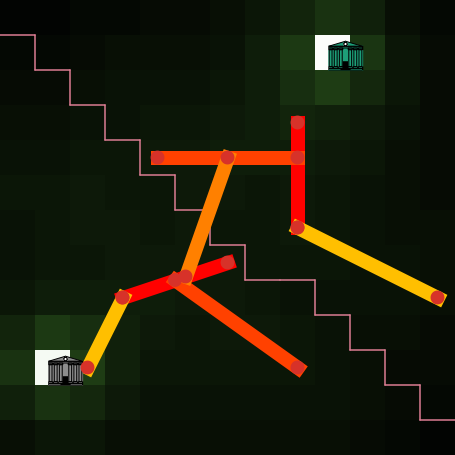
\includegraphics[width=0.5\textwidth]{Figures/PartII/Modeling/Lutecia/ex_collab_0}
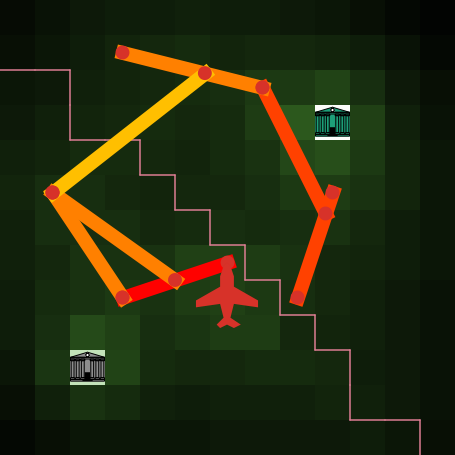
\includegraphics[width=0.5\textwidth]{Figures/PartII/Modeling/Lutecia/ex_dc_finalCollab}\\
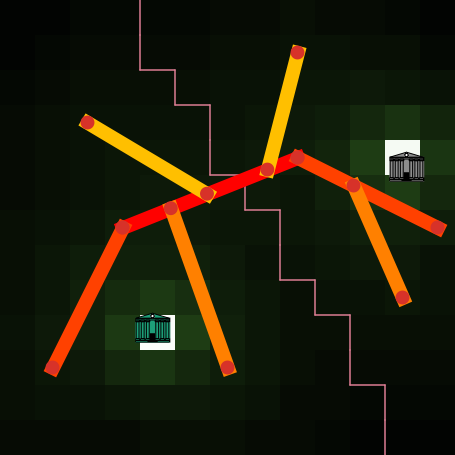
\includegraphics[width=0.5\textwidth]{Figures/PartII/Modeling/Lutecia/ex_simpleNash_0}
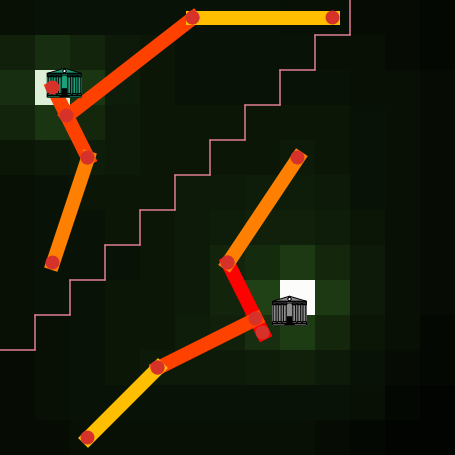
\includegraphics[width=0.5\textwidth]{Figures/PartII/Modeling/Lutecia/example_nocollab_0}
\caption[Examples of final configurations]{Examples of final configurations, with or without externality, for different values of cooperation parameters.}
\label{fig:luteciaexample}
\end{figure}
%%%%%%%%%%


%%%%%%%%%%
\begin{figure}
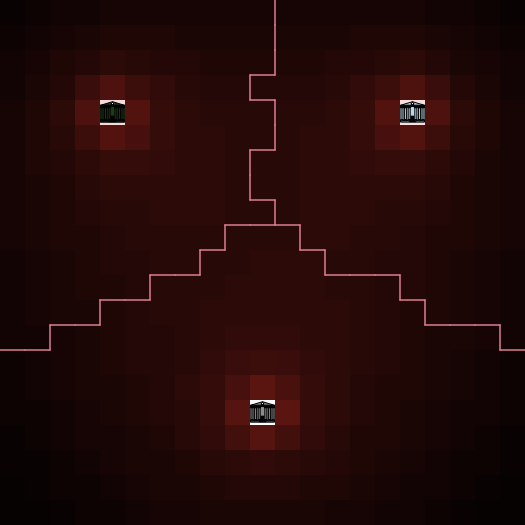
\includegraphics[width=0.5\textwidth]{Figures/PartII/Modeling/Lutecia/_MEAN_ACC}
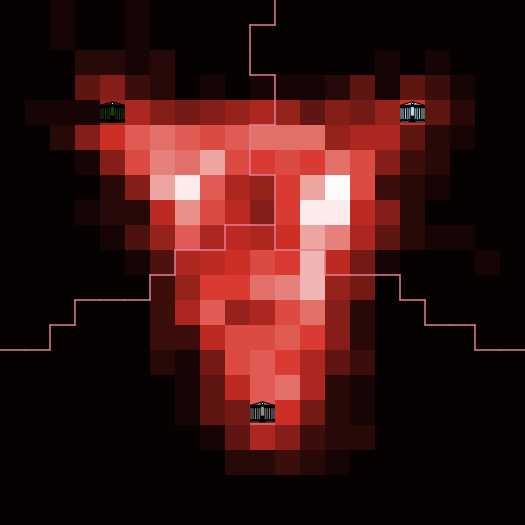
\includegraphics[width=0.5\textwidth]{Figures/PartII/Modeling/Lutecia/_NW_FREQ}
\caption[Validation of network exploration heuristic]{Validation of network exploration heuristic : mean accessibility(left) and network positions on 500 realizations on the same initial configuration. The optimal distribution of network validates network generation heuristic.}
\label{fig:luteciavalid}
\end{figure}
%%%%%%%%%%%



\subsubsection{Exploration and Validation}

We show in Fig.~\ref{fig:luteciaexample} and Fig.\ref{fig:luteciavalid} examples of obtained configurations and preliminary validation of governance and network growth heuristic. Internal validation and external validation through stylized facts, and model explorations, including statistical analysis of model behavior, are provisory for now and not presented here (see~\cite{le2015modeling} for preliminary results).


%\subsection{Perspectives}
% why is this model useful for the following









